\documentclass{beamer}
\usepackage[utf8]{inputenc}
\usepackage{graphicx}
\usetheme{Antibes}
\title{Sentiment Analysis, News \& CAC40}
\author{Alexis Daboville}
\institute{Trinity College Dublin}
\date{\today}

\begin{document}
	\begin{frame}
		\titlepage
	\end{frame}

	\begin{frame}{Introduction}
		\begin{itemize}
			\item Sentiment analysis
			\pause \item News
			\pause \item CAC40
		\end{itemize}
	\end{frame}

	\begin{frame}{Sentiments?}
		\begin{itemize}
			\item Opinions
			\item Subjectives
			\item Not facts
		\end{itemize}

		\pause

		\begin{itemize}
			\item Positive: \emph{``This film is {\color{green}great}.''}
			\item Negative: \emph{``This is a {\color{red}disaster}.''}
		\end{itemize}
	\end{frame}

	\begin{frame}{Sentiment Frequency}
		\begin{eqnarray*}
			words(day) &=& \textrm{A list of all words in the news of day}\\
			positive\_set &=& positive\_words\_set - economic\_words\_set\\
			positive\_words(day) &=& \sum_{w \in words(day)} \begin{cases}1 & \textrm{ if }w \in positive\_set\\ 0 & \mbox{ otherwise }\end{cases}\\
			positive\_freq(day) &=& \frac{length(positive\_words(day))}{length(words(day))}
		\end{eqnarray*}

		\pause

		Same method for negative sentiments.

	\end{frame}

	\begin{frame}{CAC40}
		\begin{itemize}
			\item Main French stock index
			\item 40 of the most important French companies (e.g. Total, Sanofi, BNP Paribas)
		\end{itemize}
	\end{frame}

	\begin{frame}{News Data: Problems}
		\begin{itemize}
			\item Data from several sources
			\item Paid archives
			\item \emph{Complex} systems to crawl
		\end{itemize}
	\end{frame}

	\begin{frame}{News Data: Solutions}
		\begin{itemize}
			\item Lexis Nexis (online library with numerous archives)
			\item Watir
		\end{itemize}
	\end{frame}

	\begin{frame}{News Data: Results}
		\begin{itemize}
			\item 500.000+ news
			\item From 9 economic newspapers/websites
		\end{itemize}
	\end{frame}

	\begin{frame}{CAC40 Data}
		\begin{itemize}
			\item Downloaded from Yahoo! Finance
		\end{itemize}
	\end{frame}

	\begin{frame}{Dictionaries}
		\begin{itemize}
			\item GI Dictionnary
			\item French translation by Stéphane Kazmierczak
			\pause \item Improvements:
				\begin{itemize}
					\item Removes words that carry no sentiments (too much used, no sentiments in an economic context)
					\item Stemming
				\end{itemize}
		\end{itemize}
	\end{frame}

	\begin{frame}
		\begin{figure}
			\caption{CAC40 close over time}
			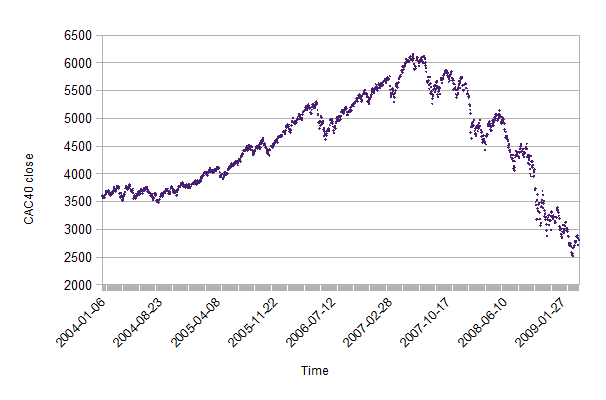
\includegraphics[scale=.5]{plots/time/cac.png}
		\end{figure}
	\end{frame}

	\begin{frame}
		\begin{figure}
			\caption{Positive sentiments frequency over time}
			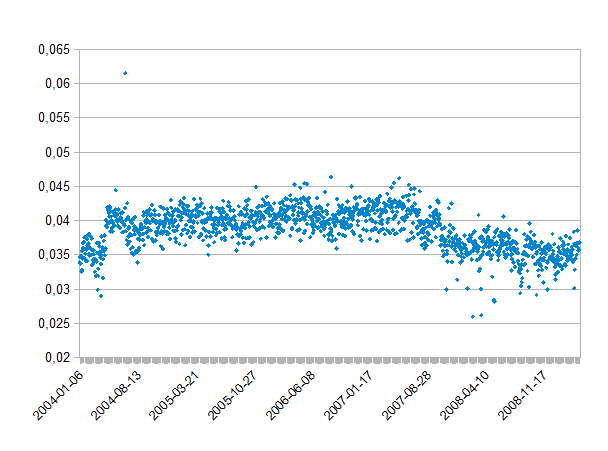
\includegraphics[scale=.5]{plots/time/pos.png}
		\end{figure}
	\end{frame}

	\begin{frame}
		\begin{figure}
			\caption{Negative sentiments frequency over time}
			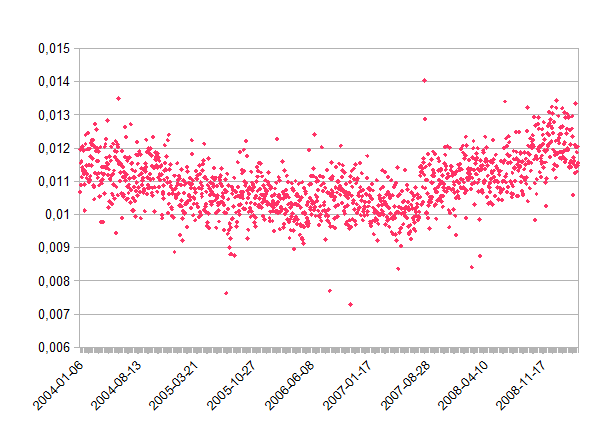
\includegraphics[scale=.5]{plots/time/neg.png}
		\end{figure}
	\end{frame}

	\begin{frame}
		\begin{figure}
			\caption{$\dfrac{positive\ sentiments\ frequency}{negative\ sentiments\ frequency}$ over time}
			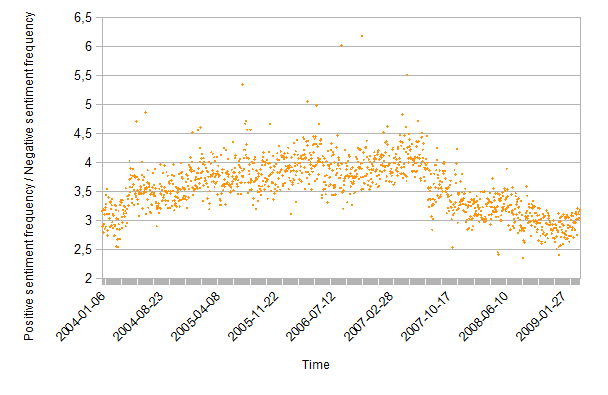
\includegraphics[scale=.5]{plots/time/posdivneg.png}
		\end{figure}
	\end{frame}

	\begin{frame}{Wrapping up}
		\begin{table}
		\scalebox{.75}{
		\begin{tabular}{|c | c | c | c|}
			\hline
			& Before mid-2007 & Mid-2007 & After mid-2007\\
			\hline
			CAC40 close & $\nearrow$ & $\rightarrow$ $\searrow$ & $\searrow$\\
			\hline
			Positive sentiments frequency & $\rightarrow$ & $\searrow$ & $\rightarrow$\\
			\hline
			Negative sentiments frequency & $\searrow$ & $\rightarrow$ & $\nearrow$\\
			\hline
			$\dfrac{Positive\ sentiments\ frequency}{Negative\ sentiments\ frequency}$ & $\nearrow$ $\rightarrow$ & $\searrow$ & $\searrow$\\
			\hline
		\end{tabular}}
		\caption{CAC40 and sentiments trends\label{trends}}
		\end{table}
	\end{frame}
	
	\begin{frame}{Returns \& Volatility}
		\begin{itemize}
			\item $return = \ln\frac{V_f}{V_i}$
			\pause \item Volatility: standard deviation of return 
		\end{itemize}
	\end{frame}
\end{document}
